
\documentclass{article}

\usepackage[left=2cm,right=2cm, top=2cm, bottom = 2cm]{geometry}
\usepackage{amsfonts}

\usepackage{amsmath}
\usepackage{xcolor}

\usepackage{tikz}
\usepackage{subfigure}



\pagestyle{empty}

\setlength{\tabcolsep}{15pt}


\newcommand{\deriv}[3][]{\frac{\mathrm{d}^{#1}#2}{\mathrm{d}#3^{#1}}}
\newcommand{\diff}{\;\mathrm{d}}

\newcommand{\norm}[1]{\left|\kern-1pt\left|#1\right|\kern-1pt\right|}




\begin{document}

\title{Fourier Sine Series}
\date{}

\maketitle
\thispagestyle{empty}

\Large

\textbf{\underline{Objective: To understand how a periodic function can be}}

\textbf{\underline{approximated by a series of sinusoids.}}






\vspace{5mm}



\textbf{Recap/Warm-up: Orthonormal Decompositions:}\bigskip



Consider functions on the interval $[0,L]$ (for some fixed, positive constant $L$), with the inner product given by
\[\langle\psi\mid\phi\rangle=\frac{2}{L}\int_0^L \psi(x)\phi(x)\diff x.\]

\begin{enumerate}
	\item Show that, for any positive integers $n$ and $m$,
		\[\left\langle \sin\left(\frac{2\pi nx}{L}\right)\Bigg|\sin\left(\frac{2\pi mx}{L}\right)\right\rangle=\delta_{nm},\]
		where $\delta$ is the Kronecker delta symbol. In other words, show that the functions $s_n(x)=\sin\left(\frac{2\pi nx}{L}\right)$ for positive integers $n$ are orthonormal.
	\item Let $f(x)$ be the step function defined by
		\[f(x)=\begin{cases}
				-1: & 0\leq x\leq \frac{L}{2}\\
				1: & \frac{L}{2}<x\leq L
			\end{cases}.\]
		\begin{enumerate}
			\item For $n\geq 1$, show that $\langle f \mid s_{2n}\rangle=0$.
			\item For $n\geq 1$, show that
				\[\langle f\mid s_{2n-1}\rangle = \frac{-2}{\pi(2n-1)}.\]
			\item Hence write down an expression for the best approximation $f_{2N-1}$ to $f$ by a linear combination of $s_0,\hdots,s_{2N-1}$, in the form
				\[f_{2N-1}(x) = \sum_{n=1}^N a_n s_{(2n-1)}(x).\]
				Graphs of $f_{2N-1}$ for various values of $N$ are shown overleaf.
		\end{enumerate}
\end{enumerate}




\clearpage




\begin{center}
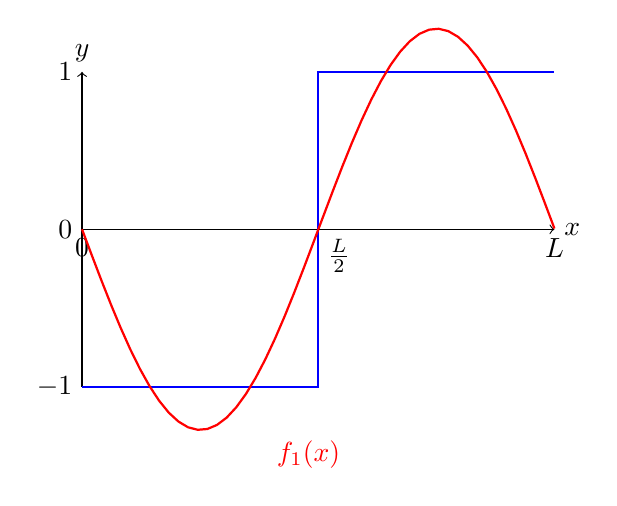
\begin{tikzpicture}
	\draw[->] (0,0) -- (6,0);
	\node[right] at (6,0) {$x$};
	\draw[->] (0,-2) -- (0,2);
	\node[above] at (0,2) {$y$};
	
	\draw[thick,blue] (0,-2) -- (3,-2) -- (3,2) -- (6,2);
	\node[below] at (0,0) {0};
	\node[below right] at (3,0) {$\frac{L}{2}$};
	\node[below] at (6,0) {$L$};
	\node[left] at (0,0) {0};
	\node[left] at (0,-2) {$-1$};
	\node[left] at (0,2) {1};
	
	\draw[thick,red,domain=0:6,samples=50] plot (\x, { - (8/3.14)*sin(6.28*\x/6 r) });
	
	\node[below,red] at (current bounding box.south) { $f_1(x)$ };
\end{tikzpicture}
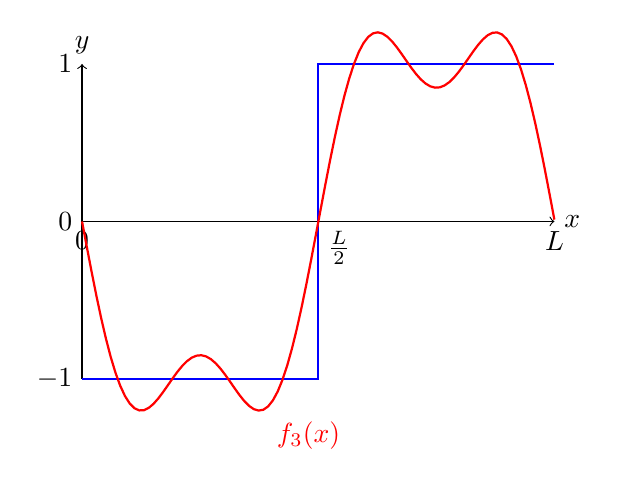
\begin{tikzpicture}
	\draw[->] (0,0) -- (6,0);
	\node[right] at (6,0) {$x$};
	\draw[->] (0,-2) -- (0,2);
	\node[above] at (0,2) {$y$};
	
	\draw[thick,blue] (0,-2) -- (3,-2) -- (3,2) -- (6,2);
	\node[below] at (0,0) {0};
	\node[below right] at (3,0) {$\frac{L}{2}$};
	\node[below] at (6,0) {$L$};
	\node[left] at (0,0) {0};
	\node[left] at (0,-2) {$-1$};
	\node[left] at (0,2) {1};
	
	\draw[thick,red,domain=0:6,samples=100] plot (\x, { - (8/3.14)*sin(6.28*\x/6 r) - (8/(3*3.14))*sin(6.28*3*\x/6 r)});
	
	\node[below,red] at (current bounding box.south) { $f_3(x)$ };
\end{tikzpicture}

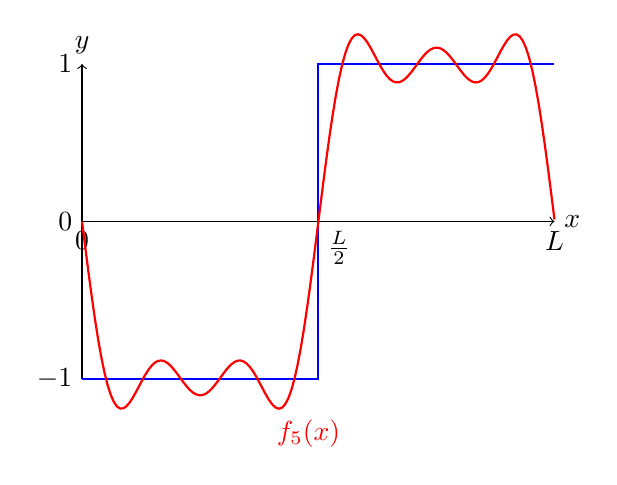
\begin{tikzpicture}
	\draw[->] (0,0) -- (6,0);
	\node[right] at (6,0) {$x$};
	\draw[->] (0,-2) -- (0,2);
	\node[above] at (0,2) {$y$};
	
	\draw[thick,blue] (0,-2) -- (3,-2) -- (3,2) -- (6,2);
	\node[below] at (0,0) {0};
	\node[below right] at (3,0) {$\frac{L}{2}$};
	\node[below] at (6,0) {$L$};
	\node[left] at (0,0) {0};
	\node[left] at (0,-2) {$-1$};
	\node[left] at (0,2) {1};
	
	\draw[thick,red,domain=0:6,samples=150] plot (\x, { - (8/3.14)*sin(6.28*\x/6 r) - (8/(3*3.14))*sin(6.28*3*\x/6 r) - (8/(5*3.14))*sin(6.28*5*\x/6 r) });
	
	\node[below,red] at (current bounding box.south) { $f_5(x)$ };
\end{tikzpicture}
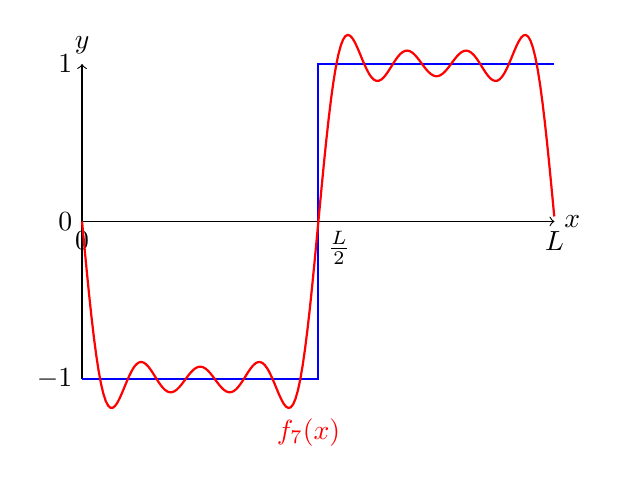
\begin{tikzpicture}
	\draw[->] (0,0) -- (6,0);
	\node[right] at (6,0) {$x$};
	\draw[->] (0,-2) -- (0,2);
	\node[above] at (0,2) {$y$};
	
	\draw[thick,blue] (0,-2) -- (3,-2) -- (3,2) -- (6,2);
	\node[below] at (0,0) {0};
	\node[below right] at (3,0) {$\frac{L}{2}$};
	\node[below] at (6,0) {$L$};
	\node[left] at (0,0) {0};
	\node[left] at (0,-2) {$-1$};
	\node[left] at (0,2) {1};
	
	\draw[thick,red,domain=0:6,samples=200] plot (\x, { - (8/3.14)*sin(6.28*\x/6 r) - (8/(3*3.14))*sin(6.28*3*\x/6 r) - (8/(5*3.14))*sin(6.28*5*\x/6 r) - (8/(7*3.14))*sin(6.28*7*\x/6 r) });
	
	\node[below,red] at (current bounding box.south) { $f_7(x)$ };
\end{tikzpicture}

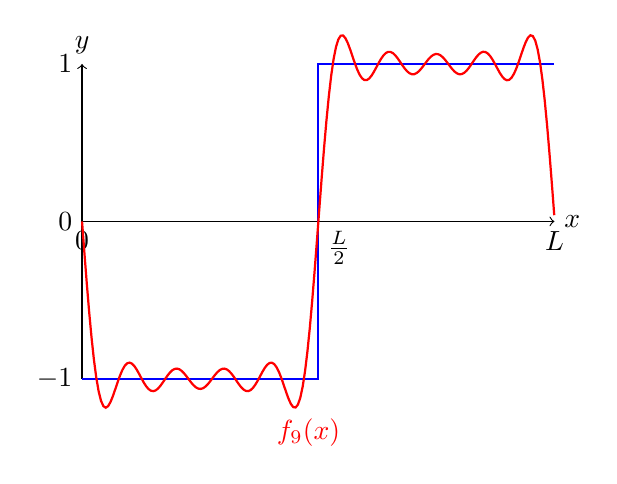
\begin{tikzpicture}
	\draw[->] (0,0) -- (6,0);
	\node[right] at (6,0) {$x$};
	\draw[->] (0,-2) -- (0,2);
	\node[above] at (0,2) {$y$};
	
	\draw[thick,blue] (0,-2) -- (3,-2) -- (3,2) -- (6,2);
	\node[below] at (0,0) {0};
	\node[below right] at (3,0) {$\frac{L}{2}$};
	\node[below] at (6,0) {$L$};
	\node[left] at (0,0) {0};
	\node[left] at (0,-2) {$-1$};
	\node[left] at (0,2) {1};
	
	\draw[thick,red,domain=0:6,samples=200] plot (\x, { - (8/3.14)*sin(6.28*\x/6 r) - (8/(3*3.14))*sin(6.28*3*\x/6 r) - (8/(5*3.14))*sin(6.28*5*\x/6 r) - (8/(7*3.14))*sin(6.28*7*\x/6 r) - (8/(9*3.14))*sin(6.28*9*\x/6 r) });
	
	\node[below,red] at (current bounding box.south) { $f_9(x)$ };
\end{tikzpicture}
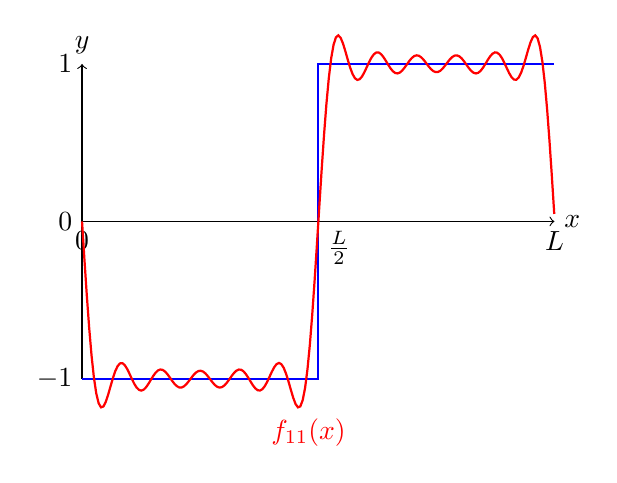
\begin{tikzpicture}
	\draw[->] (0,0) -- (6,0);
	\node[right] at (6,0) {$x$};
	\draw[->] (0,-2) -- (0,2);
	\node[above] at (0,2) {$y$};
	
	\draw[thick,blue] (0,-2) -- (3,-2) -- (3,2) -- (6,2);
	\node[below] at (0,0) {0};
	\node[below right] at (3,0) {$\frac{L}{2}$};
	\node[below] at (6,0) {$L$};
	\node[left] at (0,0) {0};
	\node[left] at (0,-2) {$-1$};
	\node[left] at (0,2) {1};
	
	\draw[thick,red,domain=0:6,samples=200] plot (\x, { - (8/3.14)*sin(6.28*\x/6 r) - (8/(3*3.14))*sin(6.28*3*\x/6 r) - (8/(5*3.14))*sin(6.28*5*\x/6 r) - (8/(7*3.14))*sin(6.28*7*\x/6 r) - (8/(9*3.14))*sin(6.28*9*\x/6 r) - (8/(11*3.14))*sin(6.28*11*\x/6 r) });
	
	\node[below,red] at (current bounding box.south) { $f_{11}(x)$ };
\end{tikzpicture}

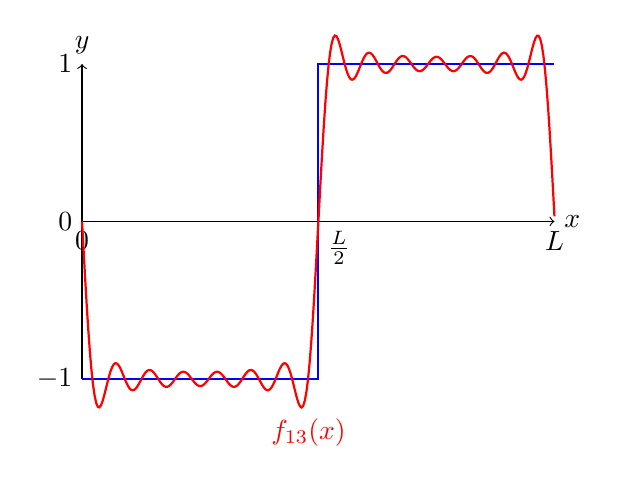
\begin{tikzpicture}
	\draw[->] (0,0) -- (6,0);
	\node[right] at (6,0) {$x$};
	\draw[->] (0,-2) -- (0,2);
	\node[above] at (0,2) {$y$};
	
	\draw[thick,blue] (0,-2) -- (3,-2) -- (3,2) -- (6,2);
	\node[below] at (0,0) {0};
	\node[below right] at (3,0) {$\frac{L}{2}$};
	\node[below] at (6,0) {$L$};
	\node[left] at (0,0) {0};
	\node[left] at (0,-2) {$-1$};
	\node[left] at (0,2) {1};
	
	\draw[thick,red,domain=0:6,samples=300] plot (\x, { - (8/3.14)*sin(6.28*\x/6 r) - (8/(3*3.14))*sin(6.28*3*\x/6 r) - (8/(5*3.14))*sin(6.28*5*\x/6 r) - (8/(7*3.14))*sin(6.28*7*\x/6 r) - (8/(9*3.14))*sin(6.28*9*\x/6 r) - (8/(11*3.14))*sin(6.28*11*\x/6 r) - (8/(13*3.14))*sin(6.28*13*\x/6 r) });
	
	\node[below,red] at (current bounding box.south) { $f_{13}(x)$ };
\end{tikzpicture}
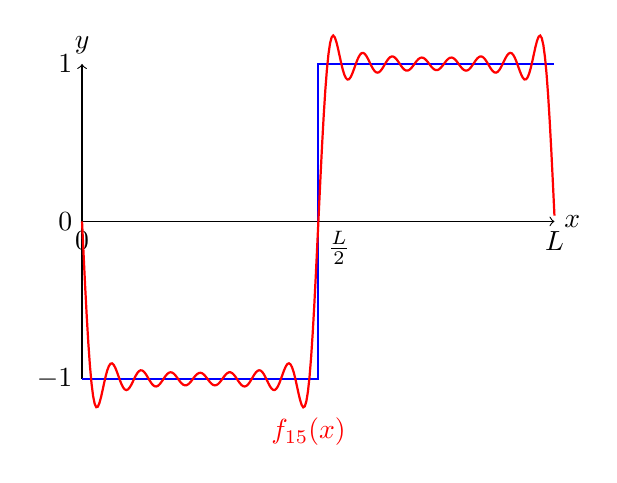
\begin{tikzpicture}
	\draw[->] (0,0) -- (6,0);
	\node[right] at (6,0) {$x$};
	\draw[->] (0,-2) -- (0,2);
	\node[above] at (0,2) {$y$};
	
	\draw[thick,blue] (0,-2) -- (3,-2) -- (3,2) -- (6,2);
	\node[below] at (0,0) {0};
	\node[below right] at (3,0) {$\frac{L}{2}$};
	\node[below] at (6,0) {$L$};
	\node[left] at (0,0) {0};
	\node[left] at (0,-2) {$-1$};
	\node[left] at (0,2) {1};
	
	\draw[thick,red,domain=0:6,samples=300] plot (\x, { - (8/3.14)*sin(6.28*\x/6 r) - (8/(3*3.14))*sin(6.28*3*\x/6 r) - (8/(5*3.14))*sin(6.28*5*\x/6 r) - (8/(7*3.14))*sin(6.28*7*\x/6 r) - (8/(9*3.14))*sin(6.28*9*\x/6 r) - (8/(11*3.14))*sin(6.28*11*\x/6 r) - (8/(13*3.14))*sin(6.28*13*\x/6 r) - (8/(15*3.14))*sin(6.28*15*\x/6 r) });
	
	\node[below,red] at (current bounding box.south) { $f_{15}(x)$ };
\end{tikzpicture}


\end{center}








\clearpage















\textbf{Theory: Fourier Sine Series:}

\bigskip



We showed in the warm up that on the interval $[0,L]$, the functions and $s_n(x)=\sin\left(\frac{2\pi nx}{L}\right)$ for $n\geq 1$ are orthonormal with respect to an integral inner product. Therefore any function $f(x)$ on the interval $[0,L]$ can be approximated by a linear combination of these:
\[f(x)\approx \sum_{n=0}^N \langle f\mid s_n\rangle s_n(x).\]

The error in this approximation cannot get larger as we take more terms (after all, we can always take the coefficients of extra terms to be 0, so an approximation with more terms can never be worse, though it might not be any better). So we are interested in taking ever larger numbers of terms, and therefore the limit as $N$ tends to infinity. We define the \textbf{Fourier sine series} of $f$ to be the function
\[f_\mathrm{sin} (x) = \sum_{n=1}^\infty \langle f\mid s_n\rangle s_n(x).\]

For any $n\geq 1$, we have
\[\langle f\mid s_n(x)\rangle s_n(x) = \frac{2}{L}\int_0^L f(x)\sin\left(\frac{2\pi nx}{L}\right)\diff x \times \sin\left(\frac{2\pi nx}{L}\right).\]

Therefore it is customary to define
\[b_n=\frac{2}{L}\int_0^L f(x)\sin\left(\frac{2\pi nx}{L}\right)\diff x,\]
and then write the Fourer sine series as
\[f_\mathrm{sin}(x)=\sum_{n=1}^\infty b_n\sin\left(\frac{2\pi nx}{L}\right).\]

We have only considered approximating a function $f$ over an interval $[0,L]$. We can extend to an interval $[a,a+L]$ simply by changing the limits on the integrals to be from $a$ to $a+L$, so intervals starting somewhere other than 0 don't change the theory.

The frequency of the sinusoid $s_n$ is called the $n^\mathrm{th}$ \textbf{harmonic}. The first harmonic (the frequency of $s_1$) is sometimes called the \textbf{fundamental frequency}.

\clearpage












\textbf{Theory: Periodic Extensions:}\bigskip


Let $f$ be a function defined on the interval $[0,L]$ (as before, any interval will do, but for convenience we assume the interval starts at 0; simply replace $x$ by $x+a$ to shift the interval by $a$). We define the \textbf{periodic extension} of $f$ to be the function $\tilde{f}$ defined on the whole real line as follows: for any $x\in\mathbb{R}$, there is some integer $n$ such that $x+nL\in[0,L]$; then $\tilde{f}(x)=f(x+nL)$. So we add $L$ to $x$ (or subtract $L$ from $x$) until it's inside the interval where $f$ is defined, then apply $f$. Whatever $f$ was, $\tilde{f}$ will be periodic, with period $L$ (unless $f$ was already periodic, with a period dividing $L$, in which case $\tilde{f}$ is just $f$).\medskip

Graph the periodic extensions of:
\begin{enumerate}
	\item The sine function on $[0,\pi]$;
	\item The cosine function on $[0,\pi]$;
	\item The Heaviside function on $[-1,1]$;
	\item The function $y=x$ on $[0,1]$.
\end{enumerate}

\bigskip


If $f$ is a function defined on $[0,L]$, then the Fourier sine series of $f$, $f_\mathrm{sin}$, is a sum of sine functions with periods dividing $L$ (the $n^\mathrm{th}$ harmonic has period $L/n$). Therefore $f_\mathrm{sin}$ is $L$-periodic. Therefore outside the interval $[0,L]$, $f_\mathrm{sin}$ approximates $\tilde{f}$, rather than $f$ itself.\medskip

For instance, take $f(x)=H\left(x-\frac{L}{2}\right)$; this is the step function from the warm-up. Sketch the graphs of $f(x)$ and $f_\mathrm{sin}(x)$ over $[-2L,2L]$.



\clearpage




\textbf{Comparison: Fourier Series and Taylor Series:}\bigskip



We have already seen one series approximation for functions, the Taylor series. There we approximated a function by polynomials, and took the limit as the degree of the polynomial approximation tended to infinity; here, we approximate a function by sinusoids of increasing frequency, and take the limit as the highest frequency used tends to infinity. Both these series approximations have their uses, and their limitations. Here we compare them in several respects.\bigskip

Firstly, what sort of function can be approximated with either series? A Taylor series requires us to differentiate the function arbitrarily many times, so is only useful for smooth functions. We saw in the warm-up a Fourier series for the step function; this is not even continuous, let alone smooth! If we take a Taylor series about a point away from the discontinuity, we simply get a constant function; so Taylor series cannot deal with the discontinuities, whereas Fourier series can.

On the other hand, a Fourier series is for a function on an interval, and extends that function periodically. So if we took a Fourier series for $e^x$, for instance, on some interval, it would be totally useless outside that interval, whereas the Taylor series is useful anywhere within the radius of convergence (which, for the exponential function, is infinite). So Fourier series are only appropriate for periodic functions, or functions where we are only interested in what happens in some bounded interval.

There is also a question of convergence for the integrals involved in the Fourier coefficients. For instance, if we take the function $x^{-3}$ on the interval $(0,1)$, we would need to integrate $x^{-3}\sin(2\pi nx)$ to find the Fourier coefficients; but this integral does not exist. On the other hand, we can Taylor expand $x^{-3}$ around $x=0.5$, have radius of convergence $0.5$, and therefore be able to approximate our function anywhere on $(0,1)$ by taking enough terms.\bigskip


Secondly, the question of accuracy of the approximation. For a Taylor series, we pick a point to expand around; the estimate is perfect \textit{at} that point, and tends to become less accurate as we move further away. On the other hand, Fourier series take a linear combination of sinusoids which minimises the area between that linear combination and the original function. So a Taylor series is a \textit{local} approximation to a function \textit{near a fixed point}, and the partial sums may become inaccurate away from that point, while a Fourier series is a \textit{global} approximation \textit{over an interval}; a partial sum may not give a particularly good approximation to the function near any particular point, but on average across the whole interval it gives the best approximation possible with the harmonics used.











\clearpage





\textbf{Practice:}\bigskip

\[f_\mathrm{sin}(x)=\sum_{n=1}^\infty b_n\sin\left(\frac{2\pi nx}{L}\right),\]
where
\[b_n = \frac{2}{L}\int_0^L f(x)\sin\left(\frac{2\pi nx}{L}\right)\diff x.\]

\begin{enumerate}
	\item Let $S(x)$ be the ``sawtooth wave'' defined by periodic extension of the function $y=x$ on the interval $[-1,1]$. Sketch the graph of $S$ and find its Fourier sine series.
	\item Let $T(x)$ be the ``triangular wave'' defined by periodic extension of the function $f(x)$, where
		\[f(x)=\begin{cases}
				x: & x\in [-1,1]\\
				2-x: & x\in [1,3].\\
			\end{cases}\]
		Sketch the graph of $T$ and find its Fourier sine series.
	\item Let $f(x)$ be the function defined by
		\[f(x)=\begin{cases}
				1: & x\in [0,\pi]\\
				-1: & x\in[\pi,2\pi].
			\end{cases}\]
		\begin{enumerate}
			\item Sketch the graph of the periodic extension of $f$ and find its Fourier sine series.
			\item Sketch the graph of the periodic extension of $f\left(x-\frac{\pi}{2}\right)$ and find its Fourier sine series. Can you explain this, and suggest an alternative to the Fourier sine series we might use?
		\end{enumerate}
\end{enumerate}


















\clearpage




{\bf Key Points to Remember:}

\vspace{5mm}

\begin{enumerate}
	\item The \textbf{Fourier sine series} of a function $f(x)$ on the interval $[a,a+L]$ is the trigonometric series
		\[f_\mathrm{sin}(x)=\sum_{n=1}^\infty b_n\sin\left(\frac{2\pi nx}{L}\right),\]
		where
		\[b_n = \frac{2}{L}\int_a^{a+L} f(x)\sin\left(\frac{2\pi nx}{L}\right)\diff x.\]
	\item The $N^\mathrm{th}$ partial sum of the Fourier sine series is the best approximation to $f$ by a linear combination of the orthonormal functions
		\[\sin\left(\frac{2\pi x}{L}\right),\hdots, \sin\left(\frac{2\pi Nx}{L}\right)\]
		(with respect to the integral inner product on $[a,a+L]$).
	\item Given a function $f$ defined on an interval $[a,a+L]$, the \textbf{periodic extension} of $f$ is the function $\tilde{f}(x)$ which agrees with $f$ on $[a,a+L]$ and repeats with period $L$.
	\item Whereas Taylor series approximate a function \textit{locally near a point}, Fourier series approximate a function \textit{globally over an interval}. There might not be any point where a Fourier approximation looks like the original function, but it approximates the function well \textit{on average}. A Taylor expansion, by contrast, approximates a function well near the basepoint, but may approximate it less and less accurately the further away from the basepoint you move.
\end{enumerate}









\end{document}